As shown in figure \ref{table:query_results}, the system is able to handle the simple case for object querying very reasonably. 
The fastest calculating predicate is \texttt{isTouching}, followed closely by \texttt{near}.
Because these two predicates operate on similar algorithms, it make sense that the two operate in similar time.
One potential significance is the fact that \texttt{isTouching} operates faster than \texttt{near}, and the only tangible difference between the two algorithms is the fact that \texttt{isTouching} has a smaller threshold than \texttt{near}.
It was first speculated that this meant that the internal Blender functions relied on by these predication functions' run-time increased with object distance.
However, the more likely explanation is the calculation of the threshold between the two functions.
In \texttt{near}, the threshold is calculated with a function that operates in linear time.
In \texttt{isTouching}, it is a constant, predetermined value, and thus requires no overhead to calculate.

The program worked into the Cornell Cup's Haptek team, where it was used to simulate a person navigating a virtual maze.  
This project set out to equip a room with several Kinect cameras which monitored the movement of a person in the room. A program, receiving input from the cameras, would build a virtual maze in a virtual representation of the room. The person's virtual avatar would be inserted into this simulation. 

The person's motion would be tracked with the cameras, and the avatar would move with the user. If the avatar came into contact with one of the virtual walls in the maze, then a buzzing feedback mechanism would be triggered. This allows the user to navigate a virtual maze. Because this is a simulation in 3D space, the project utilized many of the aspects of the \TDS project, including several of the predicates, the models for ``person'' and ``wall,'' and the temporal updating feature of the 3D scene.

In a similar note, the use of Blender has opened up a number of options for future endeavors. Because Blender is a widely-used program with a broad range of applications and widespread compatibility, \TDS has the potential to be utilized in any number of studies and situations. For example, many 3D printers currently accept model input in file formats supported by Blender. At this year's Rochack Hackathon, we were able to 3D print one of the models. This model can be seen in figure \ref{fig:3D_Print}.

\begin{figure}[h]
	\begin{center}
		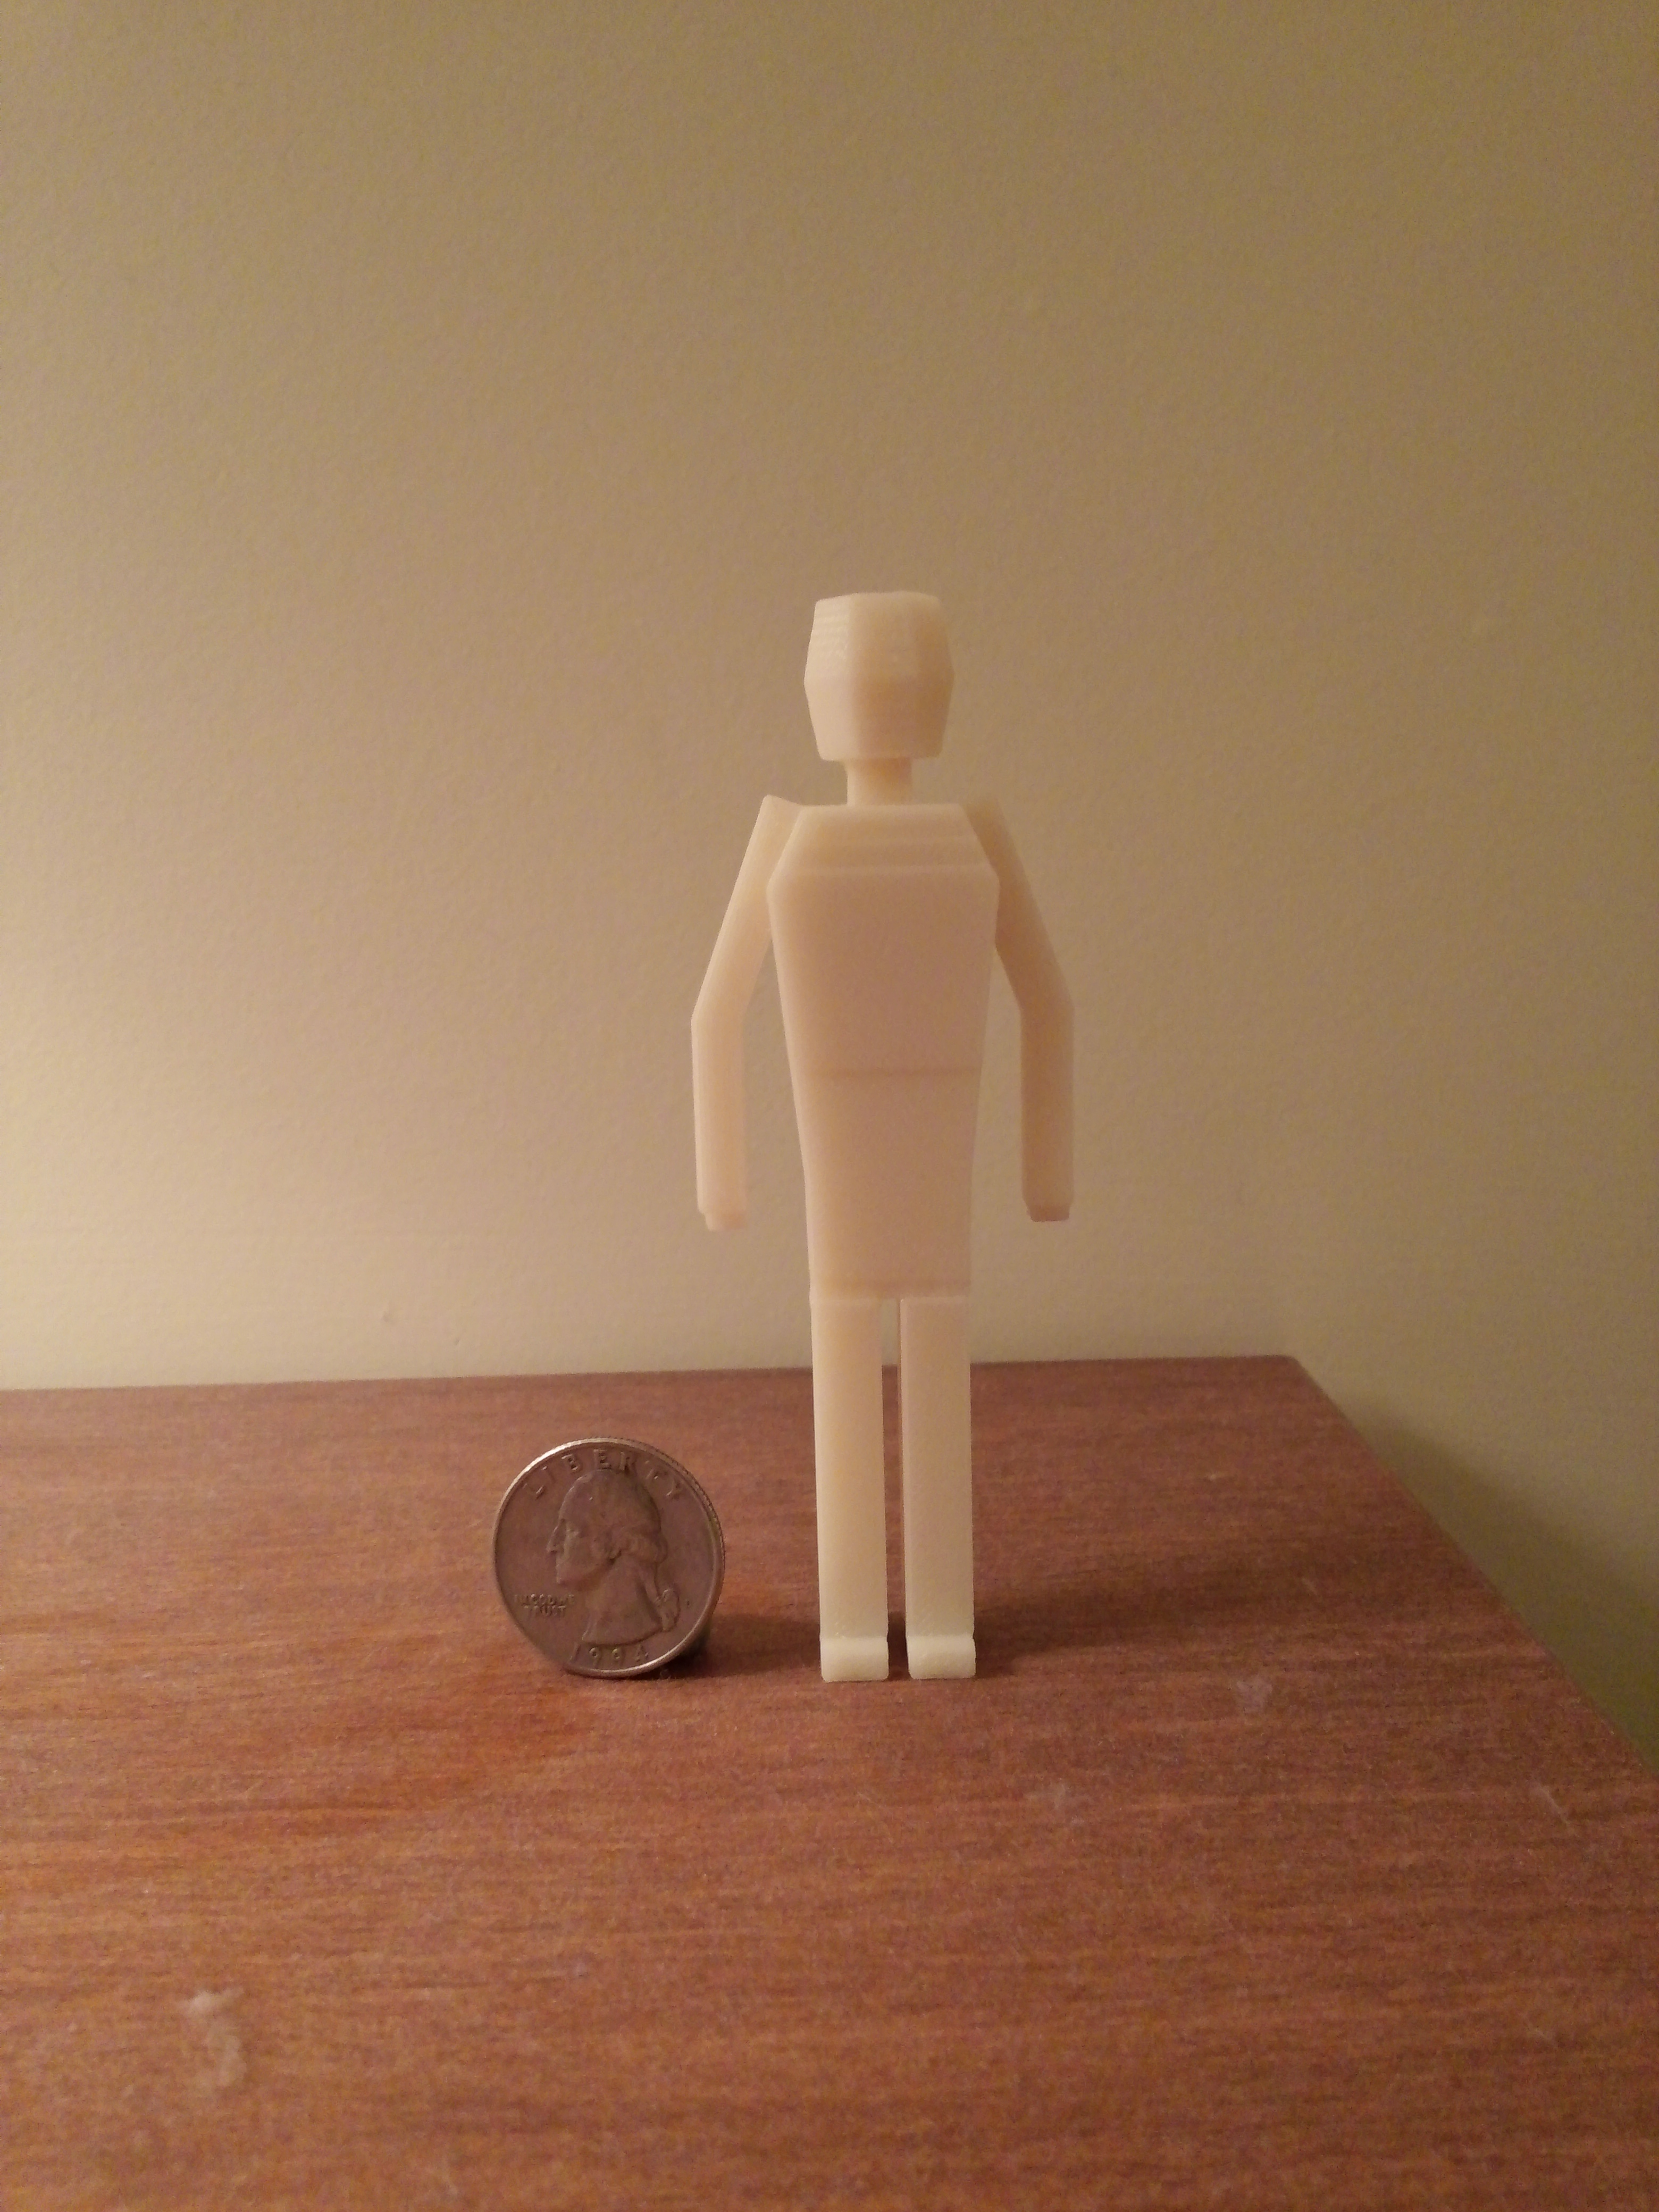
\includegraphics[width=0.45\textwidth]{figures/3D_Print.jpg}
	\end{center}
	\caption{The 3D printed model of the person from the story scene. A quarter is shown nearby for scale}
	\label{fig:3D_Print}
\end{figure} 

The Blender file for the person was uploaded with minimal changes to the 3D printer at the school, and printed. The entire process of converting the file, uploading it to the printer, and printing the figure took less than an hour. Given the growing importance of 3D printing in the present, and the many applications to 3D environments that \TDS offers, the ability to quickly model objects that can be 3D printed could prove to be a valuable feature of the system.

An area of concern is the run-time of the ``inside'' predication.
The run-time of this predication is significantly worse than the others. Because this function runs in $O(n^2)$ time, it is most likely not due to an inefficient algorithm. Rather, this lack of satisfiability is likely related to the legal placement area generated by the placement function in predMethods.py.

Inside is similar to in, differing only in that it requires one object to be inside the mesh (rather than bounding box) of the other. The legal area, however, is generated to encompass the entire bounding box. As such, it may overestimates the legal area by a considerable amount. Shrinking the placement area would potentially solve this problem, though it may prevent placement in legal areas. 

Our project was able to successfully query and place entities under predicate constraints. Because the scene was able to pass the original test of constructing the story-based image and deduce the implicit, spatial information in the scene (the person could not see the egg in the nest), the study was a success. The efficacy of rejection sampling in the placement function requires further investigation. Current testing indicates that it improves scene construction by making placements more accurate, though the key issue in this endeavor is the efficiency of the inside predicate.

The placement system creates a complex relationship between predications and entities during placement. An ``optimal'' order of placement emerges in complex scenes. Deviation from the optimal layout was shown to increase placement time dramatically.

The ``optimal'' configuration is one in which the entities are placed in order of decreasing number of predication constraints. For example, in the placement of the story scene, the required predications are:
\begin{center}
	\begin{itemize}
		\item a person is under a tree
		\item a nest is in a tree
		\item an egg is in the nest
		\item the person can see the nest
	\end{itemize}
\end{center} 
In this scene, the nest is the most constrained object, because it is used in a predication with the person (can see), the egg (in), and the tree (in). The least constrained entities are the tree and the person, each involved in only one predication. This forms a ``constraint hierarchy.'' 

For an optimal placement run-time, the entities in the scene should be placed from the most to least constrained. Placing the most constrained entities first allows the most legal placement area for the subsequent entities (which, because they are lower in the hierarchy, have naturally less constrained placement areas), which means that the system has to do less sampling and backtracking on average in order to place them.
Note that a constraint hierarchy is not necessarily unique for a given scene because multiple entities can be involved in the same number of predications.

The greatest flaw in the system, and the biggest boundary to continued expansion of the project, is the ad-hoc nature of the predicate and object database. 
Both entities and predicates are created in an ad-hoc fashion; there exist no templates for either, although some share similar features. 
Because of this, adding new members to either library can be cumbersome. 
Further, because the predicate functions of each are based on qualitative semantic interpretations of the predicates, it can be quite difficult to write functions that objectively represent the predicates they are meant to.

Our project's success in creating and querying 3D scenes demonstrates both its usability as a situation for reasoning in 3D spaces, and the expressive power of the system in general. 
Our program was able to quickly and efficiently manage and query over a small library of entities and predicates. 
The system is black-boxed to outside input, and as such can be used for more than just Epilog. Preliminary work with the 3D printed model and the collaboration with Haptek has shown this. The system, in its current form, holds potential to be of use in a number of projects and experiments that involve 3D space. We hope that the \TDS will be put to use as a specialist program, both in Epilog and beyond.